\documentclass{article}
\usepackage{geometry}
\usepackage{parskip}
\usepackage{graphicx}
\graphicspath{ {./images/} }

\geometry{
  a4paper,
  margin=1in
}

\title{SC4002}

\author{
  Ng Tze Kean\\
  \texttt{U2121193J} \and
  Ng Woon Yee\\
  \texttt{U1234567J} \and
  Yap Shen Hwei\\
  \texttt{U1234567J} \and
  Lim Boon Hien\\
  \texttt{U1234567J} \and
  Phee Kian Ann\\
  \texttt{U1234567J} \and
  Lim Ke En\\
  \texttt{U2122069L}
}
\date{\today}

\begin{document}

\maketitle

\section*{Introduction}
We will structure this report to discuss the following parts in each section,
and we detail some of the challenges that we faced and how we have overcome
them.

\section*{Part 0}

In part 0
% TODO: part 0

\section*{Part 1}

\subsubsection*{Discussion}

In this part, we prepare the word embeddings for the downstream tasks in the
later part. Before we obtain the word embeddings, we are tasked to process the
training text, mainly to find out the vocabulary size and out-of-vocabulary
(OOV) words. To start off, we first used a simple regex approach from GPT2 to
extract the tokens from the text. We then compared the tokenization process
with the NLTK tokenizer and found that the NLTK tokenizer is more accurate in
tokenizing the text.

% TODO: Add more details on the tokenization process and comparison

With that in mind, we decided to use the NLTK tokenizer to tokenize the text.
Next, we opted to use GloVe as the word embeddings for this task. A simple
extraction of the vocabulary size of GloVe is easily done though iterating and
extracting the keys of the embeddings.

To obtained the OOV words, we compared the vocabulary of the training data with
the vocabulary of GloVe through a set difference operation.

\subsubsection*{Answer to questions}

\begin{enumerate}
  \item Vocabulary Size: The vocabulary size formed from our training data is [insert
            vocabulary size]. This was calculated by [describe the method used to calculate
            vocabulary size, e.g., using Python's set function].

  \item Out-of-Vocabulary (OOV) Words: We identified [number of OOV words]
        out-of-vocabulary words in our training data. These words were present in the
        training data but not found in the [Word2vec or GloVe] dictionary

  \item Mitigating OOV Limitations: To mitigate the issue of OOV we first considered
        the use of <UNK> token to represent all OOV words. However, this approach may
        not be ideal as it does not capture the semantics of the OOV words. Instead, we
        decided to to use character-level embeddings to represent OOV words, this is
        seen in FastText where each word is broken down into character n-grams. This
        approach allows us to capture valid words that might not be in the vocabulary.

        We showcase the snippet of the <UNK> token code below:

\begin{verbatim}
for word in extended_vocab:
idx = word2idx[word]
# if word is in glove vocab, use glove vector
if word in glove_dict:
    embedding_matrix[idx] = glove_dict[word]
else:
    # use random vector for unknown words
    if word == UNK_TOKEN:
        embedding_matrix[idx] = np.random.normal(
            scale=0.6,
            size=(EMBEDDING_DIM,)
            )
    else:
        embedding_matrix[idx] =\
            embedding_matrix[word2idx[UNK_TOKEN]]
\end{verbatim}

\end{enumerate}

\section*{Part 2}

\subsubsection*{Discussion}

\subsubsection*{Answer to questions}

\section*{Part 3}

\subsubsection*{Discussion for 1}

As stated by the task, we unfreeze the word embeddings of the RNN model, allowing
for updates as the model trains. This is done by setting the trainable parameter
of the embedding layer to True.

\subsubsection*{Answer to question 1}

% attach image of accuracy and loss graph

\subsubsection*{Discussion for 2}

We apply the mitigation of OOV words by first using the <UNK> token to represent
all OOV words. Tokens from the train data that are in the GloVe dictionary will
have the embedding taken, and those that are not will be removed from the vocabulary
allowing it to be implicitly represented by the <UNK> token. The <UNK> token 
will have a random embedding generated for it.

Next, for the embedding layer, we handle the OOV words by setting the embedding
to the <UNK> token embedding.

\subsubsection*{Answer to question 2}

\subsubsection*{Discussion for 3.1}

\subsubsection*{Answer to question 3.1}

\subsection*{Discussion for 3.2 - BiGru Model}
BiGRU model stands for Bidirectional Gated Reccurent Unit, which is a type of recurrent neural network (RNN). Similarly to LSTM, GRU is designed to model sequential data by allowing information to be selectively remembered or forgotten over time. However, in GRU, the memory cell state is replaced with a "candidate activation vector", which is updated using two gates: the reset gate and update gate. The reset gate determines how much of the previous hidden state to forget while the update gate determines how much of the candidate activation vector to incorporate into the new hidden state. 

Therefore, the GRU consists of two gates:
\begin{itemize}
    \item Update gate z that selects whether the hidden state is to be updated with a new hidden state. 
    \item Reset gate that decides whether previous hidden state is ignored. 
\end{itemize}

In this implementation, Spatial dropout is used. The spatial dropout will zeroes out the entire 1D feature map from the embedding feature vector of each word, helping in regularisation. 

After the GRU layer, we will concatenate both, the average pooling and max pooling of the hidden representation and the last hidden state of GRU in order to prevent our model from forgetting informations. 
\begin{figure}
    \centering
    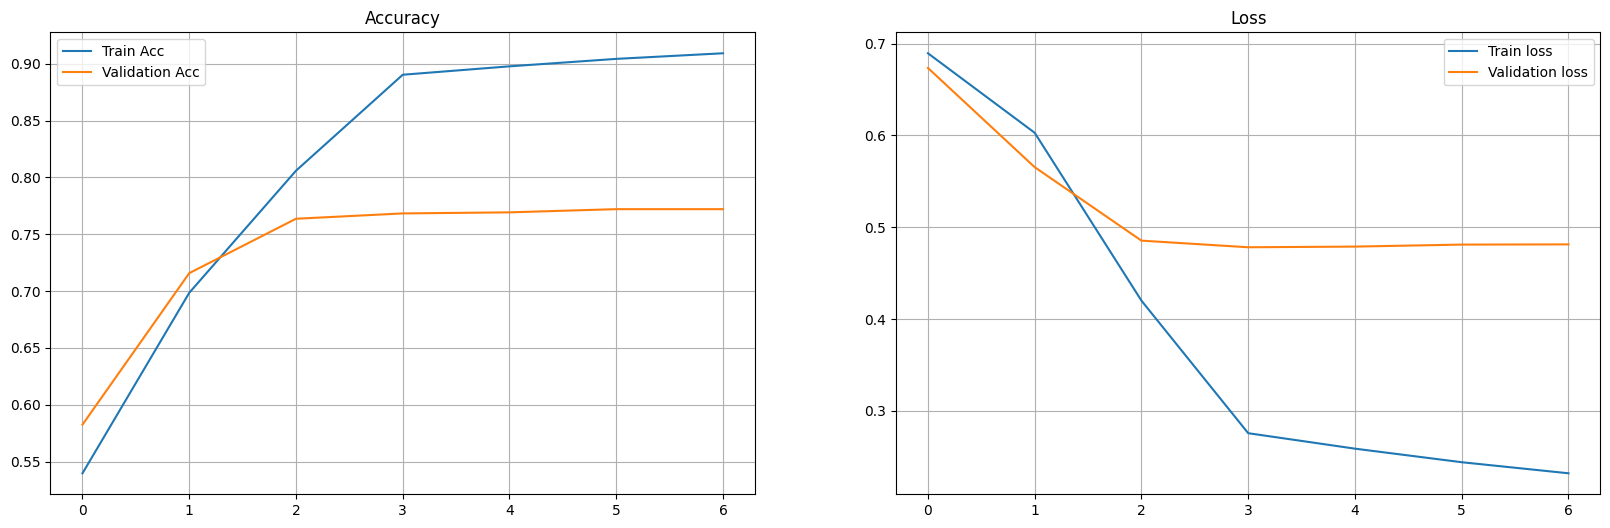
\includegraphics[width=1\linewidth]{BiGRU.png}
    \caption{Accuracy and Loss Data}
    \label{fig:enter-label}
\end{figure}

\subsection*{Answer to question 3.2}
Accuracy scores of BiLSTM and BiGRU model: 
\begin{center}
\begin{tabular}{ | c | c | }
\hline
 Model & Test Accuracy \\
\hline
 BiLSTM & [bilstm accuracy] \\
\hline
 BiGRU & 0.7992 \\
\hline
\end{tabular}
\end{center}

Compare the accuracy between BiGRU and BiLSTM

\subsubsection*{Discussion for 4}

\subsubsection*{Answer to question 4}

\section*{Conclusion}
% ...

\end{document}